% Font options: 10pm, 11pt, 12pt
% Align headings left instead of center: nocenter
\documentclass[xcolor=x11names,compress]{beamer}\usepackage[]{graphicx}\usepackage[]{color}
%% maxwidth is the original width if it is less than linewidth
%% otherwise use linewidth (to make sure the graphics do not exceed the margin)
\makeatletter
\def\maxwidth{ %
  \ifdim\Gin@nat@width>\linewidth
    \linewidth
  \else
    \Gin@nat@width
  \fi
}
\makeatother

\definecolor{fgcolor}{rgb}{0.345, 0.345, 0.345}
\newcommand{\hlnum}[1]{\textcolor[rgb]{0.686,0.059,0.569}{#1}}%
\newcommand{\hlstr}[1]{\textcolor[rgb]{0.192,0.494,0.8}{#1}}%
\newcommand{\hlcom}[1]{\textcolor[rgb]{0.678,0.584,0.686}{\textit{#1}}}%
\newcommand{\hlopt}[1]{\textcolor[rgb]{0,0,0}{#1}}%
\newcommand{\hlstd}[1]{\textcolor[rgb]{0.345,0.345,0.345}{#1}}%
\newcommand{\hlkwa}[1]{\textcolor[rgb]{0.161,0.373,0.58}{\textbf{#1}}}%
\newcommand{\hlkwb}[1]{\textcolor[rgb]{0.69,0.353,0.396}{#1}}%
\newcommand{\hlkwc}[1]{\textcolor[rgb]{0.333,0.667,0.333}{#1}}%
\newcommand{\hlkwd}[1]{\textcolor[rgb]{0.737,0.353,0.396}{\textbf{#1}}}%
\let\hlipl\hlkwb

\usepackage{framed}
\makeatletter
\newenvironment{kframe}{%
 \def\at@end@of@kframe{}%
 \ifinner\ifhmode%
  \def\at@end@of@kframe{\end{minipage}}%
  \begin{minipage}{\columnwidth}%
 \fi\fi%
 \def\FrameCommand##1{\hskip\@totalleftmargin \hskip-\fboxsep
 \colorbox{shadecolor}{##1}\hskip-\fboxsep
     % There is no \\@totalrightmargin, so:
     \hskip-\linewidth \hskip-\@totalleftmargin \hskip\columnwidth}%
 \MakeFramed {\advance\hsize-\width
   \@totalleftmargin\z@ \linewidth\hsize
   \@setminipage}}%
 {\par\unskip\endMakeFramed%
 \at@end@of@kframe}
\makeatother

\definecolor{shadecolor}{rgb}{.97, .97, .97}
\definecolor{messagecolor}{rgb}{0, 0, 0}
\definecolor{warningcolor}{rgb}{1, 0, 1}
\definecolor{errorcolor}{rgb}{1, 0, 0}
\newenvironment{knitrout}{}{} % an empty environment to be redefined in TeX

\usepackage{alltt}
%\documentclass[xcolor=x11names,compress,handout]{beamer}
\usepackage[]{graphicx}
\usepackage[]{color}
\usepackage{booktabs}
\usepackage{hyperref}
\usepackage{tikz}
\usepackage{multirow}
\usepackage{multicol}
\usepackage{dcolumn}
\usepackage{bigstrut}
\usepackage{amsmath} 
\usepackage{xcolor,colortbl}
\usepackage{amssymb}
%\newcommand{\done}{\cellcolor{teal}#1}

%% Beamer Layout %%%%%%%%%%%%%%%%%%%%%%%%%%%%%%%%%%
\useoutertheme[subsection=false,shadow]{miniframes}
\useinnertheme{default}
\usefonttheme{serif}
\usepackage{Arev}
\usepackage{pdfpages}

\setbeamerfont{title like}{shape=\scshape}
\setbeamerfont{frametitle}{shape=\scshape, size=\normalsize}

\definecolor{dkblue}{RGB}{0,0,102}

\setbeamercolor*{lower separation line head}{bg=dkblue} 
\setbeamercolor*{normal text}{fg=black,bg=white} 
\setbeamercolor*{alerted text}{fg=red} 
\setbeamercolor*{example text}{fg=black} 
\setbeamercolor*{structure}{fg=black} 
 
\setbeamercolor*{palette tertiary}{fg=black,bg=black!10} 
\setbeamercolor*{palette quaternary}{fg=black,bg=black!10} 

\renewcommand{\(}{\begin{columns}}
\renewcommand{\)}{\end{columns}}
\newcommand{\<}[1]{\begin{column}{#1}}
\renewcommand{\>}{\end{column}}

\setbeamertemplate{navigation symbols}{} 
\setbeamertemplate{footline}[frame number]
\setbeamertemplate{caption}{\raggedright\insertcaption\par}

\setbeamersize{text margin left=5pt,text margin right=5pt}

\AtBeginSection{\frame{\sectionpage}}
\usepackage{xcolor}
\hypersetup{
    colorlinks,
    linkcolor={red!50!black},
    citecolor={blue!50!black},
    urlcolor={blue!80!black}
}

\setbeamercolor{block title}{use=structure,fg=white,bg=structure.fg!75!orange}
\setbeamercolor{block body}{parent=normal text,use=block title,bg=block title.bg!10!bg}

%%%%%%%%%%%%%%%%%%%%%%%%%%%%%%%%%%%%%%%%%%%%%%%%%%



\title{FLS 6441 - Methods III: Explanation and Causation}
\subtitle{Week 5 - Natural Experiments}
\author{Jonathan Phillips}
\date{April 2019}
\IfFileExists{upquote.sty}{\usepackage{upquote}}{}
\begin{document}  

\frame{\titlepage}

\begin{frame}
\frametitle{Classification of Research Designs}
\footnotesize
\begin{table}[htbp]
  \centering
    \begin{tabular}{|p{2.3cm}|p{2.5cm}|p{2.5cm}|}
    \hline
          & \multicolumn{1}{p{2.5cm}|}{\textbf{Independence of Treatment Assignment?}} & \multicolumn{1}{p{2.5cm}|}{\textbf{Researcher Controls Treatment Assignment?}} \bigstrut\\
    \hline
    \textbf{Controlled Experiments} & \checkmark      & \checkmark  \bigstrut\\
    \hline
    \textbf{Natural Experiments} & \checkmark      &  \bigstrut\\
    \hline
    \textbf{Observational Studies} &       &  \bigstrut\\
    \hline
    \end{tabular}%
  \label{tab:addlabel}%
\end{table}%
\normalsize
\end{frame}


\begin{frame}
\frametitle{Classification of Research Designs}
\footnotesize
\begin{table}[htbp]
  \centering
  \scalebox{0.7}{
    \begin{tabular}{|p{2.2cm}|p{5cm}|c|c|}
    \hline
          &       & \multicolumn{1}{p{2.4cm}|}{\textbf{Independence of Treatment Assignment}} & \multicolumn{1}{p{3cm}|}{\textbf{Researcher Controls Treatment Assignment?}} \bigstrut\\
    \hline
    \multicolumn{1}{|p{2.9cm}|}{\multirow{2}[4]{2.9cm}{\textbf{Controlled Experiments}}} & Field Experiments & \checkmark      & \checkmark  \bigstrut\\
\cline{2-4}          & Survey and Lab Experiments &  \checkmark     & \checkmark \bigstrut\\
    \hline
          &       &       &  \bigstrut\\
    \hline
    \multicolumn{1}{|p{2.9cm}|}{\multirow{3}[6]{2.9cm}{\textbf{Natural Experiments}}} & Natural Experiments &  \checkmark     &  \bigstrut\\
\cline{2-4}          & Instrumental Variables & \checkmark      &  \bigstrut\\
\cline{2-4}          & Discontinuities & \checkmark      &  \bigstrut\\
    \hline
          &       &       &  \bigstrut\\
    \hline
    \multicolumn{1}{|p{2.9cm}|}{\multirow{4}[8]{2.9cm}{\textbf{Observational Studies}}} & Difference-in-Differences &       &  \bigstrut\\
\cline{2-4}          & Controlling for Confounding &       &  \bigstrut\\
\cline{2-4}          & Matching &       &  \bigstrut\\
\cline{2-4}          & Comparative Cases and Process Tracing &       &  \bigstrut\\
    \hline
    \end{tabular}}%
  \label{tab:addlabel}%
\end{table}%
\normalsize
\end{frame}

\section{Natural Experiments}

\begin{frame}
\frametitle{Natural Experiments}
\begin{itemize}
\item \textbf{Advantages:}
\begin{itemize}
\item We don't need to run our own experiment!
\pause
\item Still have independence of potential outcomes from treatment
\pause
\item Treatment may be more 'realistic' than in a controlled experiment
\pause
\end{itemize}
\item \textbf{Disadvantages:}
\begin{itemize}
\item We can never be sure randomization worked
\pause
\item We don't get to choose the treatments we want to evaluate
\pause
\item We don't get to choose the population and sample
\end{itemize}
\end{itemize}
\end{frame}

\begin{frame}
\frametitle{Verifying Randomization}
\begin{itemize}
\item Causal Process Observations
\end{itemize}
\end{frame}

\begin{frame}
\frametitle{The Problem of not picking your own treatment}
\begin{itemize}
\item -
\end{itemize}
\end{frame}

\section{Randomized}

\begin{frame}
\frametitle{Ferraz and Finan (2008)}
\begin{itemize}
\item Does accountability also work for negative politician performance like corruption?
\pause
\item But corruption is hard to manipulate ethically
\pause
\item What is the inferential problem of using observational data on corruption?
\pause
\item We can also look at voters' \textit{information} about corruption 
\pause
\item What is the inferential problem of using information on corruption?
\end{itemize}
\end{frame}

\begin{frame}
\frametitle{Ferraz and Finan (2008)}
\begin{itemize}
\item \textbf{Population:} Brazilian municipalities with population less than 450,000
\item \textbf{Sample:} 373 Municipalities with audits either side of 2004 elections and first-term mayors
\item \textbf{Treatment:} CGU Audit before election
\item \textbf{Control:} Audit after election
\item \textbf{Treatment Assignment Mechanism:} Randomized (Caixa)
\item \textbf{Outcome:} Vote Share for the Incumbent
\end{itemize}
\end{frame}

\begin{frame}
\frametitle{Ferraz and Finan (2008)}
\begin{itemize}
\item Methodology
\begin{itemize}
\item $IncumbVoteShare_{ms} = \alpha + \beta AuditedEarly_{ms} + X_{ms} + FE_{s} + \epsilon_{ms}$
\pause
\item NO EFFECT
\end{itemize}
\end{itemize}
\end{frame}

\begin{frame}
\frametitle{Ferraz and Finan (2008)}
\begin{itemize}
\item The importance of a theoretical model:
\begin{enumerate}
\item The content of the information released varies
\item People's expectations/priors vary
\item For reports to have an effect, voters must receive it through the media
\end{enumerate}
\item It's the interaction of expectations and information content that matters
\end{itemize}
\end{frame}

\begin{frame}
\frametitle{Ferraz and Finan (2008)}
\begin{itemize}
\item Methodology
\begin{itemize}
\item So expected results are \textit{conditional on content of the audit report}
\pause
\item $IncumbVoteShare_{ms} = \alpha + \beta AuditedEarly_{ms} + \beta_2 Corruption_{ms} + \beta_3 AuditedEarly_{ms}*Corruption_{ms} + X_{ms} + FE_{s} + \epsilon_{ms}$
\end{itemize}
\end{itemize}
\end{frame}

\begin{frame}
\frametitle{Ferraz and Finan (2008)}
\begin{itemize}
\item Results
\begin{itemize}
\item Strong corruption information (2 violations) reduces re-election by 7\% points
\item Stronger corruption information (3 violations) reduces re-election by 14\% points
\item Strong corruption information (2 violations) with local radio reduces re-election by 11\% points
\end{itemize}
\end{itemize}
\end{frame}

\begin{frame}
\begin{center}
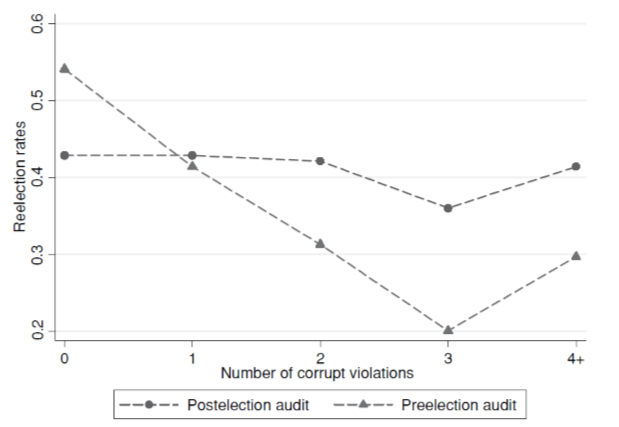
\includegraphics[scale=0.45]{Chart_FF.png}
\end{center}
\end{frame}

\begin{frame}
\frametitle{Ferraz and Finan (2008)}
\begin{itemize}
\item Did randomization work?
\item Excludability: Is treatment the same in pre/post-election audits?
\item Are corruption measures exogenous?
\end{itemize}
\end{frame}

\section{Non-Randomized}

\begin{frame}
\frametitle{Non-Randomized Natural Experiments}
\begin{itemize}
\item How can we achieve causal inference without randomization?
\pause
\item Our assumption is always "The treatment Assignment Mechanism is independent of potential outcomes"
\pause
\item Can we find real-world treatment assignments that ignored potential outcomes?
\end{itemize}
\end{frame}

\begin{frame}
\frametitle{Posner (2004)}
\begin{itemize}
\item How can we achieve causal inference without randomization?
\pause
\item Our assumption is always "The treatment Assignment Mechanism is independent of potential outcomes"
\pause
\item Can we find real-world treatment assignments that ignored potential outcomes?
\end{itemize}
\end{frame}

\end{document}
